\section{Acoustic phonons}\label{sec:11.1}

A dark-matter particle of \SI{100}{keV} transfers at most $2\mchi v_{\mathrm{max}} = \SI{0.53}{keV}$ of momentum. Given to a free silicon nucleus, that momentum would deposit $q^2/2M = \SI{5.4}{\micro eV}$, far below any threshold. Given to the crystal, it can create one longitudinal acoustic phonon of energy $c_{\mathrm{LA}}q \approx \SI{16}{meV}$, because the whole crystal takes up the momentum and the energy is set by the sound speed rather than by the mass of a nucleus. The kinematic match, with the momentum taken up by the whole crystal and the energy set by the sound speed, makes single phonons the channel of the lightest dark matter that couples to nucleons (\cref{sec:1.3}). At long wavelengths the single-phonon rate depends on the material only through the sound speeds, and for a light mediator it is the same for every material.

\subsection{The one-phonon response}

Take a dark-matter particle that couples to protons and neutrons with the same potential $\tilde V_N(\vect{q})$, the spin-independent coupling $\mathcal{O}_1$ of \cref{sec:8.1}. By \cref{eq:8.1-nuclear}, a nucleus of species $\kappa$ then carries the coupling $A_\kappa\tilde V_N(\vect{q})F_N(q)$, and the dark matter sees the target through the single operator
\begin{equation*}
  O_N(\vect{q}) = \sum_\kappa A_\kappa\,n_\kappa(\vect{q}) ,
\end{equation*}
the nucleon number density of the crystal at momentum $\vect{q}$. The nuclear form factor $F_N$ of \cref{eq:2.2-FN} is one to better than $10^{-3}$ at the momentum transfers of this section, which stay below a few keV, and we drop it. The coupling has no electronic row, so the electrons enter only through the forces they transmit between nuclei: the phonons are those of the Born--Oppenheimer surface (\cref{sec:5.1}), and the final states lie in the electron-following sector of \cref{tab:8-sectors}. Screening, which acts on rows that couple to charge (\cref{sec:8.4}), does not enter. The dark photon, which couples to charge, is the subject of \cref{sec:11.2}.

The rate per unit target mass is \cref{eq:8.2-spectrum} with one row, $\mathfrak{D} = |\tilde V_N(\vect{q})|^2$ and $S = S_A$. Here $\omega_{\vect{q}} = \vect{q}\cdot\vect{v} - q^2/2\mchi$ is the energy the dark matter loses (\cref{eq:1.3-omegaq}), not a phonon frequency, and $S_A$ is the response \cref{eq:4.2-Sab} of $O_N$, the nuclear block $\sum_{\kappa\kappa'}A_\kappa A_{\kappa'}S_{\kappa\kappa'}$. The one-phonon part of $S_A$ follows from the amplitude of \cref{sec:5.3}. To first order in the displacement, a nucleus of species $\kappa$ emits a phonon $\vect{Q}\nu$ with the amplitude
\begin{equation*}
  \langle n_{\vect{Q}\nu} + 1|\,n_\kappa(\vect{q})\,|n_{\vect{Q}\nu}\rangle = \ii\,\ee^{\ii\vect{q}\cdot\vect{\tau}_\kappa}\,\frac{\vect{q}\cdot\vect{e}_{\kappa\nu}(\vect{Q})^*}{\sqrt{2M_\kappa\omega_{\vect{Q}\nu}}}\,\sqrt{N(n_{\vect{Q}\nu} + 1)}\,\sum_{\vect{G}}\delta_{\vect{q},\vect{Q} + \vect{G}} .
\end{equation*}
Keeping the full exponential of the displacement multiplies this amplitude by $\ee^{-W_\kappa(\vect{q})}$: to first order in the displacement correlation $\mathcal{C}_{\kappa\kappa'}$, the generating formula \cref{eq:5.6-gen} for a pair of nuclei is the one-phonon term with the factor $\ee^{-W_\kappa - W_{\kappa'}}$ in front. The amplitudes of the nuclei of one cell add with their phases. We square, sum over the final phonon states and divide by the volume $\Vol = N\Omega$ as in \cref{eq:4.2-Sab}. The factor $N$ cancels, and the Kronecker delta leaves in each branch one phonon wavevector $\vect{Q}$, the reduction of $\vect{q}$ to the first Brillouin zone:
\begin{keyresult}[One-phonon nuclear response]
\begin{equation}
  \begin{aligned}
  S^{(1)}_A(\vect{q},\omega) = \frac{2\pi}{\Omega}\sum_\nu{}&\frac{\bigl|\sum_\kappa A_\kappa\,\ee^{-W_\kappa(\vect{q})}\,\ee^{\ii\vect{q}\cdot\vect{\tau}_\kappa}\,\vect{q}\cdot\vect{e}_{\kappa\nu}(\vect{Q})^*/\sqrt{M_\kappa}\bigr|^2}{2\omega_{\vect{Q}\nu}} \\
  &\times\Bigl[(n_{\vect{Q}\nu} + 1)\,\delta(\omega - \omega_{\vect{Q}\nu}) + n_{\vect{Q}\nu}\,\delta(\omega + \omega_{\vect{Q}\nu})\Bigr] ,
  \end{aligned}
  \label{eq:11.1-S1}
\end{equation}
with $\vect{Q} = \vect{q} - \vect{G}$ in the first zone, $\vect{q}$ itself unreduced in the phase $\ee^{\ii\vect{q}\cdot\vect{\tau}_\kappa}$, and the phase convention of \cref{eq:5.3-u}.
\end{keyresult}
\noindent The absorption term follows from the second matrix element of \cref{eq:5.3-me}; since $\vect{e}_{\kappa\nu}(-\vect{Q}) = \vect{e}_{\kappa\nu}(\vect{Q})^*$, the modulus of the amplitude is unchanged. In a detector at \SI{10}{mK}, $n_{\vect{Q}\nu}$ vanishes for every phonon above a few tens of \si{\micro eV} (\cref{sec:5.3}), and only emission remains. On the truncation label of \cref{sec:8.5}, \cref{eq:11.1-S1} is the point $\mathcal{K}$ = one-phonon, $n_A = 0$, with $n_T = 0$ for the emission term and $n_T = 1$ for the absorption term, and $n_B = 0$ throughout.

The weight of a branch in \cref{eq:11.1-S1} is the projection of $\vect{q}$ on the displacement of each nucleus, divided by the phonon energy, so that soft modes polarized along $\vect{q}$ dominate. The momentum is conserved up to a reciprocal-lattice vector, so that each $\vect{q}$ excites one phonon per branch, with the energy fixed by the dispersion: the response is a set of sharp lines in $\omega$ at fixed $\vect{q}$. And the Debye--Waller factor $\ee^{-2W_\kappa}$ of \cref{eq:5.6-W} measures the competition with the multiphonon terms of \cref{sec:11.3}. In silicon, $2W_\kappa = q^2\langle u_x^2\rangle$ is $3\times10^{-3}$ at $q = \SI{2.25}{keV}$ with the zero-temperature $\langle u_x^2\rangle = \SI{2.45e-3}{\angstrom^2}$ of \cref{we:5-dw}, so in the first Brillouin zone the factor is one to $3\times10^{-3}$.

\subsection{The long-wavelength limit}

Most of the rate of light dark matter comes from momentum transfers well inside the first zone. For a crystal with a lattice constant of a few \si{\angstrom}, the scale of the zone is
\begin{equation}
  q_{\mathrm{BZ}} = \Bigl(\frac{6\pi^2}{\Omega}\Bigr)^{1/3} ,
  \label{eq:11.1-qBZ}
\end{equation}
the radius of a sphere with the volume of the Brillouin zone, which holds one wavevector per primitive cell. For silicon, $\Omega = a^3/4$ and $q_{\mathrm{BZ}} = \SI{1.139}{\angstrom^{-1}} = \SI{2.25}{keV}$, between the distances from $\mathrm{\Gamma}$ to L (\SI{1.98}{keV}) and to X (\SI{2.28}{keV}). The zone scale $q_{\mathrm{BZ}}$ should not be confused with the Debye wavevector $Q_{\mathrm{D}}$ of \cref{eq:5.2-debye}, which counts one wavevector per atom and is larger by $n_{\mathrm{at}}^{1/3}$.

For $q \ll q_{\mathrm{BZ}}$, \cref{sec:5.2} removes the reciprocal-lattice vector, the internal motion of the cell and the curvature of the dispersion. The reciprocal-lattice vector is $\vect{G} = 0$ and $\vect{Q} = \vect{q}$. The acoustic polarization vectors move every nucleus of the cell together, $\vect{e}_{\kappa\nu} = (M_\kappa/M_{\mathrm{cell}})^{1/2}\hat{\vect{e}}_\nu(\hat{\vect{q}})$, with $\hat{\vect{e}}_\nu$ the unit polarizations of the Christoffel problem (\cref{app:C.18}), and the dispersion is linear, $\omega_{\vect{q}\nu} = c_\nu(\hat{\vect{q}})\,q$. And the phases $\ee^{\ii\vect{q}\cdot\vect{\tau}_\kappa}$ and the Debye--Waller factors are one up to corrections of order $qa$ and $q^2\langle u_x^2\rangle$. The sum over nuclei in \cref{eq:11.1-S1} then becomes $q\,(\hat{\vect{q}}\cdot\hat{\vect{e}}_\nu)\sum_\kappa A_\kappa/\sqrt{M_{\mathrm{cell}}}$, the optical branches drop out, since the center of mass of the cell is at rest in an optical branch (\cref{sec:5.2}), and at $T = 0$
\begin{equation*}
  S^{(1)}_A(\vect{q},\omega) = \frac{\pi\,q\,A_{\mathrm{cell}}^2}{\Omega\,M_{\mathrm{cell}}}\sum_{\nu = 1}^{3}\frac{(\hat{\vect{q}}\cdot\hat{\vect{e}}_\nu)^2}{c_\nu(\hat{\vect{q}})}\,\delta\bigl(\omega - c_\nu(\hat{\vect{q}})\,q\bigr) ,
\end{equation*}
with $A_{\mathrm{cell}} = \sum_\kappa A_\kappa$ the number of nucleons in a cell. Dividing by $\rho_T = M_{\mathrm{cell}}/\Omega$ and writing the nuclear masses as $M_\kappa = A_\kappa m_u$ with $m_u = \SI{931.494}{MeV}$ the atomic mass unit gives
\begin{keyresult}[Long-wavelength acoustic structure factor]
\begin{equation}
  \frac{S^{(1)}_A(\vect{q},\omega)}{\rho_T} = \frac{\pi q}{m_u^2}\sum_{\nu = 1}^{3}\frac{(\hat{\vect{q}}\cdot\hat{\vect{e}}_\nu)^2}{c_\nu(\hat{\vect{q}})}\,\delta\bigl(\omega - c_\nu(\hat{\vect{q}})\,q\bigr) , \qquad q \ll q_{\mathrm{BZ}} .
  \label{eq:11.1-Sac}
\end{equation}
\end{keyresult}
\noindent Per unit mass, the coherent sum over the $A_{\mathrm{cell}}$ nucleons of a cell leaves a response independent of the composition. The material enters through its sound speeds and the polarizations of its acoustic branches. The weights $(\hat{\vect{q}}\cdot\hat{\vect{e}}_\nu)^2$ sum to one over the three branches, by the completeness of the polarizations, and along a symmetry direction the longitudinal branch takes all of the weight. In a general direction the polarizations of the quasi-transverse branches are not exactly perpendicular to $\hat{\vect{q}}$ (\cref{app:C.18}), and the quasi-transverse branches take a small share. The binding energy of the nuclei and the isotopic mixture make $M_\kappa/A_\kappa$ differ from $m_u$ by less than a percent, so the replacement $M_\kappa = A_\kappa m_u$ is accurate to a percent.

\begin{limitbox}[Long-wavelength acoustic structure factor][lim:11.1a]
At momentum transfers small compared with the zone, and for a coupling to nucleon number, the longitudinal acoustic branch carries the one-phonon response of a crystal per unit mass, $S/\rho_T = (\pi q/m_u^2)\,\delta(\omega - c_{\mathrm{LA}}q)/c_{\mathrm{LA}}$, the same for every composition~\cites[Eq.~(30) with Eq.~(27)]{campbelldeem2022dark}[Eq.~(10)]{campbelldeem2020multiphonon}. Off the symmetry directions the quasi-transverse branches share the weight, as in \cref{eq:11.1-Sac}.
\par\smallskip
{\centering
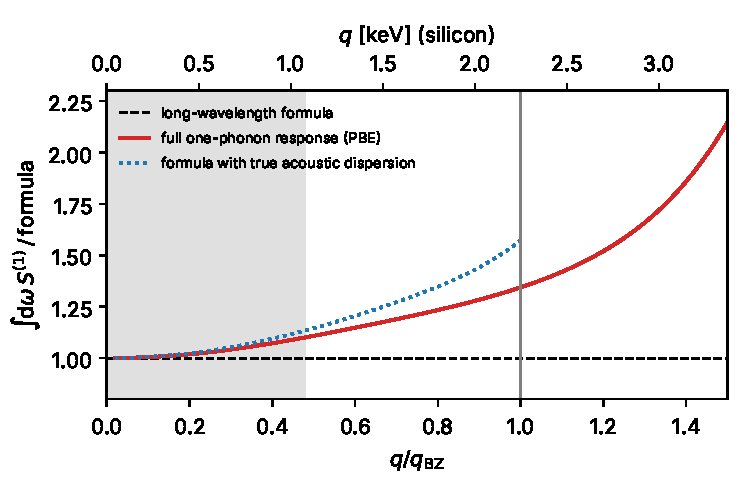
\includegraphics[width=\linewidth]{figures/ch11/limit11_1a.pdf}
\captionof{figure}{The $\omega$-integrated one-phonon response of silicon at $T = 0$, \cref{eq:11.1-S1} with all six branches, Umklapp terms and the Debye--Waller factor (solid), divided by the long-wavelength form \cref{eq:11.1-Sac} (dashed, one), both averaged over the directions of $\vect{q}$, against $q/q_{\mathrm{BZ}}$, with $q_{\mathrm{BZ}} = \SI{2.25}{keV}$. Phonons from the PBE force constants of \cref{sec:5.2}, Fourier-interpolated; the formula uses the sound speeds and polarizations of the same force constants, so that the ratio tends to one as $q \to 0$. Dotted: the long-wavelength polarizations with the true acoustic dispersion $\omega_{\vect{q}\nu}$ in place of $c_\nu q$, the leading correction. Gray: $q < 0.48\,q_{\mathrm{BZ}} = \SI{1.08}{keV}$, where the full response and the long-wavelength form agree within \SI{10}{\percent}; they agree within \SI{5}{\percent} below $0.34\,q_{\mathrm{BZ}}$. At $q_{\mathrm{BZ}}$ the formula is \SI{26}{\percent} low.}\label{fig:11-limit-a}
\par}
\smallskip
Toward the zone boundary the acoustic branches bend below $c_\nu q$, and since the weight goes as $1/\omega$, the long-wavelength form underestimates the response; beyond $q_{\mathrm{BZ}}$ the phonon carries only the reduced momentum, and the response grows as $q^2$, the incoherent form of \cref{sec:11.3}.
\end{limitbox}

The dispersion accounts for most of the departure of the full response from \cref{eq:11.1-Sac} below $q_{\mathrm{BZ}}/2$; the polarizations and the phases $\ee^{\ii\vect{q}\cdot\vect{\tau}_\kappa}$ change the ratio at order $(qa)^2$ with the opposite sign. For a rate weighted toward small $q$, as with a light mediator, the region below $q_{\mathrm{BZ}}/2$ gives nearly all of the rate and the formula is accurate. For a heavy mediator the rate is weighted toward the largest $q$ that kinematics allows, $2\mchi v_{\mathrm{max}}$, and the response there stays within \SI{10}{\percent} of the formula only for masses up to about $0.48\,q_{\mathrm{BZ}}/2v_{\mathrm{max}} = \SI{0.20}{MeV}$ in silicon.

\subsection{Orientation-averaged rate}

A crystal at a fixed orientation sees the dark-matter wind from one direction, and its rate depends on that direction; this dependence is the daily modulation of \cref{sec:11.7}. For a rate averaged over the orientations of the crystal, the response enters through its average over the directions of $\vect{q}$, and the velocity integral of \cref{eq:8.2-spectrum} acts on the delta function alone. The velocity integral gives $\eta(\vmin)/2q$ per unit $\dd^3q/(2\pi)^3$, with $\eta$ the mean inverse speed of \cref{eq:1.3-eta} (\cref{sec:8.2}). For a phonon of energy $\omega = c_\nu q$ and elastic scattering, \cref{eq:1.3-vmin} gives
\begin{equation*}
  \vmin = c_\nu + \frac{q}{2\mchi} ,
\end{equation*}
the sound speed plus half the speed the dark matter loses. We write the potential as in \cref{sec:1.4}, $|\tilde V_N(q)|^2 = \pi\sigma_p\FDM(q)^2/\mu_{\chi p}^2$, with $\sigma_p$ the dark-matter--proton cross-section, $\mu_{\chi p}$ the reduced mass and $\FDM$ the form factor of \cref{eq:1.4-defs} with $q_0 = \alpha m_e$. Inserting \cref{eq:11.1-Sac} into \cref{eq:8.2-spectrum}, integrating $\omega$ above a threshold $\omega_{\mathrm{th}}$ and collecting $4\pi\cdot\pi\cdot\pi/(2(2\pi)^3) = 1/4$ gives
\begin{keyresult}[One-acoustic-phonon rate per unit mass]
\begin{equation}
  \mathcal{R} = \frac{\rho_\chi\,\sigma_p}{4\,\mchi\,\mu_{\chi p}^2\,m_u^2}\,\Bigl\langle\sum_{\nu = 1}^{3}\frac{(\hat{\vect{q}}\cdot\hat{\vect{e}}_\nu)^2}{c_\nu}\int_{\omega_{\mathrm{th}}/c_\nu}^{q_{\mathrm{up},\nu}}\dd q\;q^2\,\FDM(q)^2\,\eta\Bigl(c_\nu + \frac{q}{2\mchi}\Bigr)\Bigr\rangle_{\hat{\vect{q}}} ,
  \label{eq:11.1-rate}
\end{equation}
with $c_\nu$ and $\hat{\vect{e}}_\nu$ taken at $\hat{\vect{q}}$, the brackets the average over the sphere of directions, and the upper limit $q_{\mathrm{up},\nu} = \min[2\mchi(v_{\mathrm{max}} - c_\nu),\,q_{\mathrm{BZ}}]$.
\end{keyresult}
\noindent The kinematic upper limit is where $\eta$ vanishes, $\vmin = v_{\mathrm{max}}$; the zone cut $q_{\mathrm{BZ}}$ is the range of \cref{eq:11.1-Sac}, beyond which the multiphonon response of \cref{sec:11.3} dominates. The rate is nonzero only when the lower limit lies below the upper one, $\omega_{\mathrm{th}}/c_\nu \le 2\mchi(v_{\mathrm{max}} - c_\nu)$, and this condition defines the \emph{acoustic edge} of \cref{sec:9.2},
\begin{equation}
  m_{\mathrm{min}}^{\mathrm{ac}} = \frac{\omega_{\mathrm{th}}}{2c_\nu(v_{\mathrm{max}} - c_\nu)} \simeq \frac{\omega_{\mathrm{th}}}{2c_\nu v_{\mathrm{max}}} ,
  \label{eq:11.1-edge}
\end{equation}
set by the largest speed of a branch with longitudinal weight over all directions, $c_{\mathrm{LA,max}}$. For silicon at $\omega_{\mathrm{th}} = \SI{1}{meV}$, $c_{\mathrm{LA,max}} = \SI{9.35}{km.s^{-1}}$ along $[111]$ and $m_{\mathrm{min}}^{\mathrm{ac}} = \SI{6.1}{keV}$, against \SI{0.28}{keV} for the threshold mass.

\begin{figure}[tbp]
  \centering
  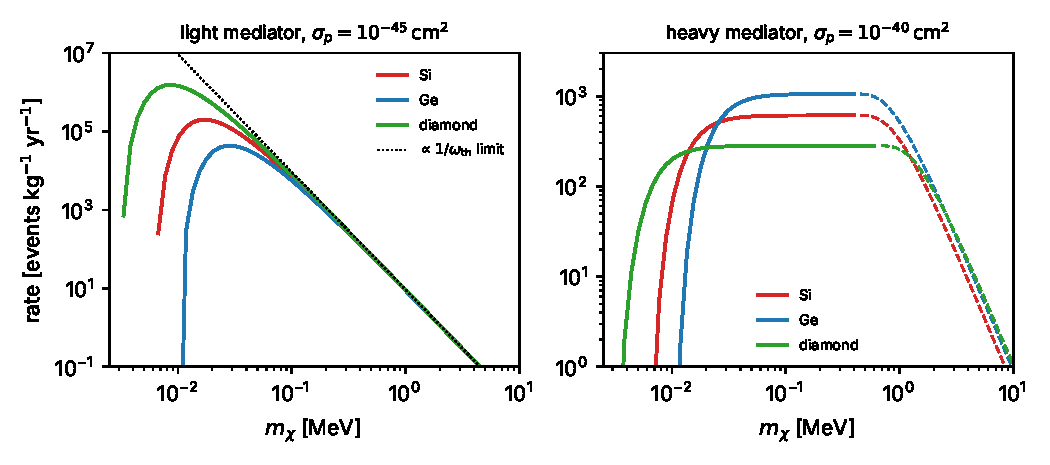
\includegraphics[width=\linewidth]{figures/ch11/fig11_1.pdf}
  \caption{Rate of single-acoustic-phonon emission per unit target mass, \cref{eq:11.1-rate}, for silicon, germanium and diamond at a threshold $\omega_{\mathrm{th}} = \SI{1}{meV}$, averaged over the orientation of the crystal, with equal couplings to protons and neutrons, $\rho_\chi = \SI{0.3}{GeV.cm^{-3}}$ and the standard halo of \cref{sec:1.2}. Sound speeds and polarizations from the Christoffel problem of the measured room-temperature elastic tensors (\cref{we:11-cbar}); momentum transfers $q \le q_{\mathrm{BZ}}$, Debye--Waller factor one. Left: light mediator, $\FDM = (q_0/q)^2$, $\sigma_p = 10^{-45}\,\mathrm{cm^2}$; dotted, the target-independent limit \cref{eq:11.1-light}. Right: heavy mediator, $\FDM = 1$, $\sigma_p = 10^{-40}\,\mathrm{cm^2}$; solid up to $q_{\mathrm{BZ}}/2v_{\mathrm{max}}$ (0.42, 0.41 and \SI{0.65}{MeV}), dashed above, where the fall is an artifact of the cut $q \le q_{\mathrm{BZ}}$ and where the multiphonon and Umklapp terms of \cref{sec:11.3} dominate. The edges are 6.1 (Si), 10.2 (Ge) and \SI{3.1}{keV} (diamond).}
  \label{fig:11-rate}
\end{figure}

\subsection{Light mediator}

For a light mediator, $\FDM^2 = (q_0/q)^4$, the integrand of \cref{eq:11.1-rate} falls as $q^{-2}$, and the rate is dominated by the smallest momentum transfer that a phonon above threshold can carry. In the variable $u = q/2\mchi$, the integral of one branch and direction is
\begin{equation*}
  \frac{q_0^4}{2\mchi}\int_{u_-}^{u_+}\dd u\,\frac{\eta(c_\nu + u)}{u^2} , \qquad u_- = \frac{\omega_{\mathrm{th}}}{2\mchi c_\nu} , \quad u_+ = v_{\mathrm{max}} - c_\nu .
\end{equation*}
Far above the edge, where $u_- \ll u_+$, the integral tends to $\eta(c_\nu)/u_-$, and since $u_- = \omega_{\mathrm{th}}/2\mchi c_\nu$, the $q$-integral of each branch and direction is $q_0^4c_\nu\eta(c_\nu)/\omega_{\mathrm{th}}$. Its factor $c_\nu$ cancels the weight $1/c_\nu$ in the brackets of \cref{eq:11.1-rate}. The shift of $\eta$ by $c_\nu$ is of relative order $c_\nu^2/v_0^2 \sim 10^{-3}$, since the laboratory speed distribution vanishes as $v^2$ at small speeds and $\eta$ is flat at the origin. By the completeness $\sum_\nu(\hat{\vect{q}}\cdot\hat{\vect{e}}_\nu)^2 = 1$ the weights of the directions and branches then add up to one, and
\begin{equation}
  \mathcal{R}_{\mathrm{light}} = \frac{\rho_\chi\,\sigma_p\,q_0^4\,\eta(0)}{4\,\mchi\,\mu_{\chi p}^2\,m_u^2\,\omega_{\mathrm{th}}} .
  \label{eq:11.1-light}
\end{equation}
The rate per unit mass is the same for every crystal, inversely proportional to the threshold, and it falls as $\mchi^{-3}$ for $\mchi \ll m_p$. The light-mediator curves of \cref{fig:11-rate} merge with \cref{eq:11.1-light} at high mass. They separate near the edges, which differ by a factor of three between diamond and germanium.

To find how far above the edge the limit \cref{eq:11.1-light} holds, write $\eta(c_\nu + u) = \eta(0) - [\eta(0) - \eta(c_\nu + u)]$. The first term integrates to $\eta(0)(1/u_- - 1/u_+)$. In the second term, the bracket vanishes as $u^2$ at small $u$, so the integral of the second term from $0$ to $u_-$ is of order $u_-$, and to first order in $u_-$ this integral can run from $0$ to $u_+$. We define
\begin{equation}
  \kappa_\eta = \frac{u_+}{\eta(0)}\int_0^{u_+}\dd u\,\frac{\eta(0) - \eta(u)}{u^2} ,
  \label{eq:11.1-kappa}
\end{equation}
and use $u_-/u_+ = m_{\mathrm{min}}^{\mathrm{ac}}/\mchi$ from \cref{eq:11.1-edge}. The integral of one branch and direction is then $(\eta(0)/u_-)[1 - (1 + \kappa_\eta)\,m_{\mathrm{min}}^{\mathrm{ac}}/\mchi]$ up to terms of second order in $m_{\mathrm{min}}^{\mathrm{ac}}/\mchi$. The rate is therefore
\begin{equation}
  \frac{\mathcal{R}}{\mathcal{R}_{\mathrm{light}}} = \Bigl[1 - (1 + \kappa_\eta)\frac{m_{\mathrm{min}}^{\mathrm{ac}}}{\mchi} + O\Bigl(\frac{m_{\mathrm{min}}^{\mathrm{ac}}}{\mchi}\Bigr)^{\!2}\Bigr] , \qquad \kappa_\eta = 3.14 ,
  \label{eq:11.1-correction}
\end{equation}
with $\mathcal{R}_{\mathrm{light}}$ the limit \cref{eq:11.1-light}, for $\mchi \le q_{\mathrm{BZ}}/2v_{\mathrm{max}}$, where the kinematic limit $u_+$ applies. The value of $\kappa_\eta$ is a property of the halo alone: it is \cref{eq:11.1-kappa} for the standard halo of \cref{sec:1.2} with $u_+ = v_{\mathrm{max}}$, the limit $c_\nu \ll v_{\mathrm{max}}$. At the sound speed of silicon, $u_+ = v_{\mathrm{max}} - c_\nu$ and $\kappa_\eta = 3.09$. The material enters only through the edge, and the term $1$ of $1 + \kappa_\eta$ is the loss of the momentum transfers above $u_+$, and the term $\kappa_\eta$ is the loss of the slow particles that the halo lacks. For a crystal the edge in \cref{eq:11.1-correction} is the average over directions and branches, weighted like the rate: this average equals $m_{\mathrm{min}}^{\mathrm{ac}}$ evaluated at the speed $\langle\sum_\nu(\hat{\vect{q}}\cdot\hat{\vect{e}}_\nu)^2/c_\nu\rangle^{-1}$, and for silicon the speed is \SI{8.956}{km.s^{-1}} (\cref{we:11-cbar}) and the edge \SI{6.39}{keV}. Above $q_{\mathrm{BZ}}/2v_{\mathrm{max}}$ the zone cut replaces $u_+$, and the bracket tends to $1 - \omega_{\mathrm{th}}/(c_\nu q_{\mathrm{BZ}})$, 0.985 for silicon at \SI{1}{meV}.

\begin{limitbox}[Light-mediator single-phonon rate][lim:11.1b]
For a light mediator the one-phonon rate per unit target mass is $\mathcal{R} = \rho_\chi\sigma_pq_0^4\eta(0)/(4\mchi\mu_{\chi p}^2m_u^2\omega_{\mathrm{th}})$, inversely proportional to the threshold and independent of the target~\cite[Eq.~(35)]{griffin2020multichannel}.
\par\smallskip
{\centering
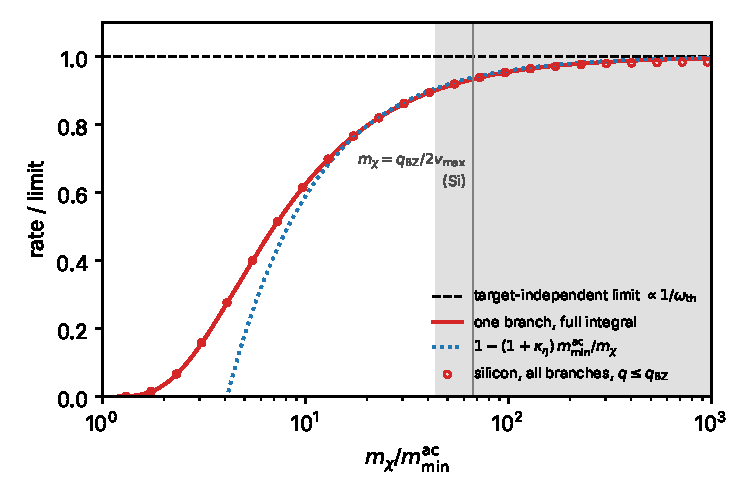
\includegraphics[width=\linewidth]{figures/ch11/limit11_1b.pdf}
\captionof{figure}{The light-mediator rate \cref{eq:11.1-rate}, divided by its target-independent limit \cref{eq:11.1-light} (dashed, one), against $\mchi/m_{\mathrm{min}}^{\mathrm{ac}}$. Solid: one branch of speed \SI{9.0}{km.s^{-1}} without the zone cut; the curve changes by \SI{3}{\percent} at $\mchi = 10\,m_{\mathrm{min}}^{\mathrm{ac}}$ between speeds of 3 and \SI{18}{km.s^{-1}}. Circles: silicon, all branches and directions, with $q \le q_{\mathrm{BZ}}$; on this axis $m_{\mathrm{min}}^{\mathrm{ac}} = \SI{6.39}{keV}$ at $\omega_{\mathrm{th}} = \SI{1}{meV}$, the edge for the polarization-weighted inverse speed \SI{8.956}{km.s^{-1}} of \cref{eq:11.1-heavy}; the vertical line marks $q_{\mathrm{BZ}}/2v_{\mathrm{max}}$, above which the zone cut holds the ratio at 0.985. Dotted: the first-order correction \cref{eq:11.1-correction} with $\kappa_\eta = 3.09$. Gray: $\mchi \ge 44\,m_{\mathrm{min}}^{\mathrm{ac}}$, where the rate is within \SI{10}{\percent} of the limit. The first-order form is within \SI{10}{\percent} of the full rate for $\mchi \ge 9\,m_{\mathrm{min}}^{\mathrm{ac}}$. Standard halo of \cref{sec:1.2}.}\label{fig:11-limit-b}
\par}
\smallskip
Within a few times the edge the momentum window $[\omega_{\mathrm{th}}/c_\nu,\,2\mchi v_{\mathrm{max}}]$ closes and only the fastest particles of the halo contribute, so the rate falls far below the limit and depends on the material through its edge.
\end{limitbox}

\begin{workedexample}{The light-mediator correction at three times the edge}\label{we:11-light}
Take silicon at $\omega_{\mathrm{th}} = \SI{1}{meV}$, where $m_{\mathrm{min}}^{\mathrm{ac}} = \SI{6.39}{keV}$ for the polarization-weighted inverse speed \SI{8.956}{km.s^{-1}} of \cref{eq:11.1-heavy}, and $\mchi = 3\,m_{\mathrm{min}}^{\mathrm{ac}} = \SI{19.2}{keV}$. The momentum transfers that can create a phonon above threshold run from $\omega_{\mathrm{th}}/c = \SI{33}{eV}$ to $2\mchi(v_{\mathrm{max}} - c) = \SI{100}{eV}$, a factor of three. With $\kappa_\eta = 3.09$ at this sound speed, the first-order factor is $1 - 4.09/3 = -0.36$: negative, and therefore meaningless. The full integral of \cref{eq:11.1-rate}, with all branches and directions, gives $\mathcal{R}/\mathcal{R}_{\mathrm{light}} = 0.149$. The expansion behind \cref{eq:11.1-correction} has failed at this mass, because the speeds that contribute, $\vmin$ between $c + u_-$ and $v_{\mathrm{max}}$, all lie in the tail of the halo above \SI{270}{km.s^{-1}}, where $\eta$ is far from flat. At ten times the edge, \SI{63.9}{keV}, the full ratio is 0.625 and the first-order form 0.591; at 44 times, \SI{0.28}{MeV}, the full ratio is 0.902 and the first-order form 0.907. The target-independent statement holds within \SI{10}{\percent} only from about \SI{0.28}{MeV} in silicon, and for any two materials only above 44 times the higher of their edges.
\end{workedexample}

\subsection{Heavy mediator}

For a heavy mediator, $\FDM = 1$, the integrand of \cref{eq:11.1-rate} grows as $q^2$, and the rate is dominated by the largest momentum transfer, $2\mchi(v_{\mathrm{max}} - c_\nu)$. With $u = q/2\mchi$ the integral of one branch is $8\mchi^3\int_{u_-}^{u_+}\dd u\,u^2\eta(c_\nu + u)$. Well above the edge and with $c_\nu \ll v_{\mathrm{max}}$, it tends to $8\mchi^3I_0$, with $I_0 = \int_0^{v_{\mathrm{max}}}\dd u\,u^2\eta(u) = 5.32\times10^{-7}$ for the standard halo. For $\mchi \ll m_p$ the reduced mass is $\mu_{\chi p} \approx \mchi$, and the factors of $\mchi$ cancel:
\begin{equation}
  \mathcal{R} = \frac{2\rho_\chi\,\sigma_p\,I_0}{m_u^2}\,\Bigl\langle\sum_\nu\frac{(\hat{\vect{q}}\cdot\hat{\vect{e}}_\nu)^2}{c_\nu}\Bigr\rangle_{\hat{\vect{q}}} .
  \label{eq:11.1-heavy}
\end{equation}
The rate per unit mass is independent of the dark-matter mass and inversely proportional to a polarization-weighted mean speed, so soft crystals have the larger rate. The plateaus of \cref{fig:11-rate} nearly stand in the ratio of the inverse speeds, $8.956/5.321 = 1.68$ for germanium against silicon and $8.956/18.16 = 0.49$ for diamond. The computed rates at \SI{0.3}{MeV} stand in the ratios 1.73 and 0.46. The difference between the computed ratios and the ratios of the inverse speeds comes from the shift of $\eta$ by $c_\nu$. The shift matters at the large $u$ that a heavy mediator favors, where $\eta$ is not flat, and lowers the rate of a stiff crystal by several percent per \SI{10}{km.s^{-1}}.

The plateau is reached only well above the edge and, in silicon, ends near \SI{0.42}{MeV}. Near the edge the lower cut removes part of $I_0$, and the rate approaches \cref{eq:11.1-heavy} only slowly, because $\eta$ falls steeply toward $v_{\mathrm{max}}$ and the integrand is weighted toward small $u$. In silicon the rate reaches \SI{90}{\percent} of the plateau value (654 events per kilogram and year at $\sigma_p = 10^{-40}\,\mathrm{cm^2}$) only at \SI{45}{keV}, seven times the edge. However, the silicon rate never exceeds \SI{94}{\percent} of the plateau value, and the diamond rate never exceeds \SI{87}{\percent} of its plateau value, because \cref{eq:11.1-heavy} drops the shift of $\eta$ by $c_\nu$. By \cref{fig:11-limit-a}, from about \SI{0.2}{MeV} the response at the largest momentum transfers already differs from \cref{eq:11.1-Sac} by more than \SI{10}{\percent}. Above $q_{\mathrm{BZ}}/2v_{\mathrm{max}}$, \SI{0.42}{MeV} for silicon, the momentum transfers leave the region where \cref{eq:11.1-Sac} holds, and Umklapp processes and multiphonons dominate (\cref{sec:11.3}). \Cref{sec:17.5} names the inverse of the bracket in \cref{eq:11.1-heavy} the effective sound speed of the channel and ranks materials by it.

\subsection{Sound speeds from the elastic tensor}

The rates above need the sound speeds in every direction, and with them two averages: the largest longitudinal speed for the edge and the polarization-weighted inverse speed of \cref{eq:11.1-heavy}. The speeds and both averages follow from the elastic tensor $C_{ijkl}$ and the density through the Christoffel equation \cref{eq:C.18-christoffel}: in each direction $\hat{\vect{q}}$ the eigenvalues of $\mathsf{M}_{ik} = C_{ijkl}\hat q_j\hat q_l$ are $\rho_Tc_\nu(\hat{\vect{q}})^2$, and the eigenvectors are the polarizations $\hat{\vect{e}}_\nu$ of \cref{eq:11.1-Sac}.

The elastic constants are measured or computed by density-functional theory (\cref{app:E.4}), and a computed tensor must be in the Voigt order of \cref{app:C.18} before it enters the Christoffel matrix.

\begin{workedexample}{The rate coefficient of silicon}\label{we:11-cbar}
The room-temperature constants of silicon are $C_{11} = 165.6$, $C_{12} = 63.9$ and $C_{44} = \SI{79.5}{GPa}$, with $\rho_T = \SI{2.33}{g.cm^{-3}}$ (\cref{app:C.18}). Along the three symmetry directions \cref{eq:C.18-cubic} gives $\rho_Tc_{\mathrm{LA}}^2 = 165.6$, $194.3$ and \SI{203.8}{GPa}, and $c_{\mathrm{LA}} = 8.43$, 9.13 and \SI{9.35}{km.s^{-1}} along $[100]$, $[110]$ and $[111]$. The speed varies by \SI{11}{\percent} over the sphere, and the averages need all directions.

The polarization-weighted average is a quadrature. On a product grid of Gauss--Legendre nodes in $\cos\theta$ and equally spaced nodes in $\phi$ (\cref{app:C.18}), with the $3\times3$ Christoffel matrix diagonalized at each node, the inverse of the rate coefficient of \cref{eq:11.1-heavy}, $\langle\sum_\nu(\hat{\vect{q}}\cdot\hat{\vect{e}}_\nu)^2/c_\nu\rangle^{-1}$, is \SI{8.956}{km.s^{-1}}. The same procedure yields \SI{5.321}{km.s^{-1}} for germanium and \SI{18.16}{km.s^{-1}} for diamond, from the tensors $131$, $49$, \SI{68}{GPa}~\cite{mcskimin1963elastic} and $1081$, $125$, \SI{579}{GPa}~\cite{mcskimin1972elastic}, as tabulated in Ref.~\cite[Table~III]{haxhijaj2026lattice}, with the densities 5.33 and \SI{3.52}{g.cm^{-3}} that follow from the lattice constants 5.658 and \SI{3.567}{\angstrom}.
\end{workedexample}

A tabulated speed can be tested without the full tensor. The largest eigenvalue of the Christoffel matrix is at least its expectation value in the unit vector $\hat{\vect{q}}$. For cubic symmetry that expectation value is never below the bulk modulus $B = (C_{11} + 2C_{12})/3$ of \cref{eq:C.18-bulk}, and the two inequalities give \cref{eq:C.18-rayleigh}:
\begin{equation}
  c_{\mathrm{LA}}(\hat{\vect{q}}) \ge \sqrt{B/\rho_T} \qquad\text{(cubic crystals, every direction)} .
  \label{eq:11.1-rayleigh}
\end{equation}
The bound is \SI{6.48}{km.s^{-1}} for silicon, \SI{3.79}{km.s^{-1}} for germanium and \SI{11.23}{km.s^{-1}} for diamond, 23, 24 and \SI{36}{\percent} below their slowest longitudinal speeds. It is proved for cubic crystals only; for lower symmetries the uniform compression and the uniform strain no longer coincide (\cref{app:C.18}), and the bound must be replaced by the Christoffel eigenvalue itself. \Cref{sec:17.5} applies the bound to tabulated speeds.

